\subsection{General Overview}\label{sec_res_corp}

    \paragraph{Descriptive Measures}
    
        To provide a general overview of the main corpus resulting from our methodology's Step 5, Table \ref{tab_corpora_characs} presents simple textual characteristics. The corpus consists of 573,999 tweets from 45,525 distinct Twitter users. Appendix Figure \ref{random_tweets_tot} shows four random tweets from the total corpus.
        
        
        \begin{table}[H]
            %\footnotesize
            \centering
            
            \subfile{tabs/corp_charac_main}
            
            \caption{Corpus Characteristics, Total Corpus}
            
            \floatfoot{\it 
            %Notes: Unique words and hashtags can have duplicates across the subcategories ''left-leaning'', ''right-leaning'' or ''unlabeled''.
            %\\ 
            Data Source: Retrieved from Twitter API, spanning the time frame Nov 1\textsuperscript{st}, 2020 -- April 11\textsuperscript{th}, 2022. Data is cleaned by our proposed methodology, such that the corpus includes tweets with topic-related keywords (semantic link + country contextual) and are tweeted by Twitter users in Chile or Chilean nationals and contains tweets that mainly regard the topic of immigration.}
            
            \label{tab_corpora_characs}
        \end{table}
        
        
        The tweets' distribution over time is presented in Figure \ref{total_tweets_per_day} from which three peaks are evident. The first peak is in February 2021 and coincided with a mass deportation of immigrants. The second and third peak occur in late September 2021 and late January 2022, respectively. These two peaks coincided with two violent anti-immigration protests which took place in the northern border city of Iquique.
        
        Out of the 346,600 distinct words in the corpus, Figure \ref{general_Word_Cloud} presents the most-used ones in a word cloud. As expected, it is seen that the keywords used for construction of the corpus appear prominent, for instance {\it 'inmigracion}, {\it 'inmigrantes}, and {\it 'venezolano'}. There also appears some relevant words that are strongly related with the legal situation of immigrants and the influx of immigrants, for instance {\it 'ilegales'}, {\it 'ilegal'} and {\it 'descontrolada'}. Also, the word cloud shows some common bigrams related to illegal situation like {\it 'inmigrantes, ilegales'} (Eng: Illegals, immigrant) or  {\it ‘migracion,  ilegal'} (Eng: Illegal, immigration). Interestingly, the term {\it 'terrorismo'} is prevalent and also features in multiple of the most-used bigrams in Figure \ref{fig_bi_tot}. Terrorism would not normally be considered connected to immigration in Chile. We analyze this finding further on page \pageref{par_res_terr}.
        
        \begin{figure}[H]
            \caption{Tweet Count and Word Coud, Total Corpus}
        %    \label{}
            
            \centering
                \begin{subfigure}{0.49\textwidth}
                    \caption{Tweets per Day}
                    \centering        
                    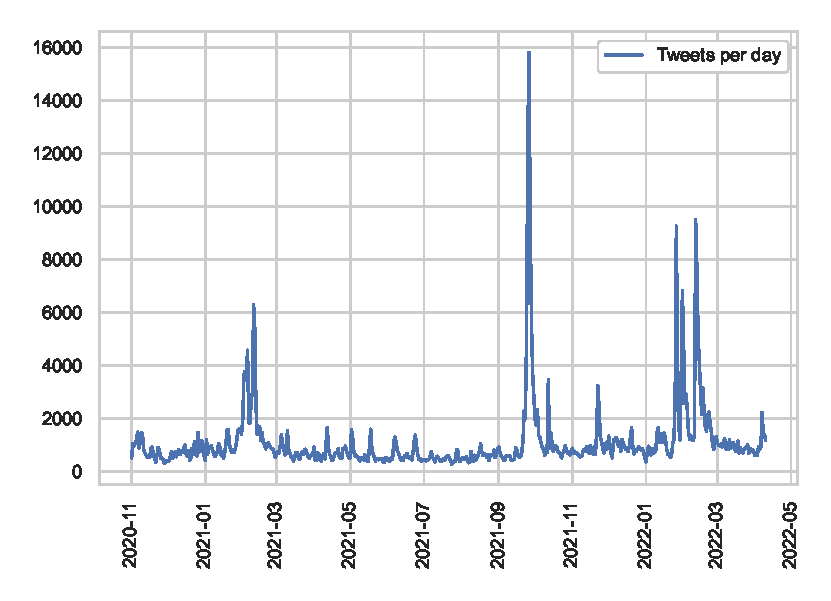
\includegraphics[width=.99\linewidth]{figs/Tweets_per_day.eps}
                    \label{total_tweets_per_day}
                \end{subfigure} %
                \begin{subfigure}{0.49\textwidth}
                    \caption{Word Cloud of Tweets}
                    \centering
                    \includegraphics[width=.99\linewidth]{figs/WordCloud_General.png}
                    \label{general_Word_Cloud}
                \end{subfigure}
           
            
            \floatfoot{\it 
                    Notes: Textual preprocessing steps in outputs include lowercase enforcement and converting Spanish special characters (e.g. á, ñ, etc.) into corresponding non-accentuated ones.
                    \vspace{0.5em} \\
                    Data Source: Retrieved from Twitter API, spanning the time frame Nov 1\textsuperscript{st}, 2020 -- April 11\textsuperscript{th}, 2022. Corpus includes tweets by Twitter users in Chile or Chilean nationals that mainly pertain to immigration. Corpus cleaned by the steps in our methodology as described in Section \ref{sec_meth_gene} and Appendix \ref{app_sec_meth}.}
        \end{figure}  
        
        
        Some of the most-used hashtags in the corpus refer to northern Chilean border cities such as \texttt{\#iquique}, \texttt{\#antofagasta} and \texttt{\#arica} as is seen from Figure \ref{fig_hash_tot}. This indicates that Chilean Twitter users are concerned about immigrants entering from the norhern border cities. This is further supported by the prominence of the hashtags \texttt{\#venezolanos} (Eng: Venezuelans) and \texttt{\#venezuela} as Venezuelan immigrants typically enter Chile from the north. To gauge whether Twitter users talk about immigrants in a negative or positive way, we consider some of the other most-used hashtags. Some hashtags are emotionally neutral such as \texttt{\#inmigrantes} (Eng: Immigration) or \texttt{\#migracion} (Eng: Migration). However, some hashtags such as \texttt{\#nomasinmigrantes} (Eng: No more immgirants) and \texttt{\#noesimmigracionesinvasion} (Eng: It's not immigration, it's invasion) carry strong negative connotations towards immigrants. We find further descriptive evidence of anti-immigratory agendas by looking at the most-used bigrams in Figure \ref{fig_bi_tot}. Here we find talking points of immigration being illegal and related to crime from the bigrams {\it 'inmigrantes, ilegales'} (Eng: Immigrants, illegals), {\it 'inmigracion, descontrolada'} (Eng: Migration, uncontrolled) and {\it 'inmigracion, delincuencia'} (Eng: Migration, crime). However, we also see signs that some Twitter users try to call out the negative speech by highlighting the xenophobic elements of the general talking points with the hashtag \texttt{\#xenofobia}. Hence, we find a general pattern of the Chilean Twittersphere being against migration, specifically concerned about illegal immigration and the crime it supposedly brings with it. Although some users seem to be against xenophobia.
        
        \begin{figure}[H]
            \caption{Top 15 Hashtags and Bigrams, Total Corpus}
            \label{fig_hash_bi_tot}
            
            \centering
                \begin{subfigure}{0.49\textwidth}
                    \caption{Top Hashtags}
                    \centering        
                    \includegraphics[width=.99\linewidth]{figs/Common_Hashtags_1.eps}
                    \label{fig_hash_tot}
                \end{subfigure} %
        %    \par\bigskip
                \begin{subfigure}{0.49\textwidth}
                    \caption{Top Bigrams}
                    \centering
                    \includegraphics[width=.99\linewidth]{figs/Common_Bigrams_1.eps}
                    \label{fig_bi_tot}
                \end{subfigure}
           
            
            \floatfoot{\it 
                    Notes: Textual preprocessing steps in outputs include lowercase enforcement and converting Spanish special characters (e.g. á, ñ, etc.) into corresponding non-accentuated ones.
                    \vspace{0.5em} \\
                    Data Source: Retrieved from Twitter API, spanning the time frame Nov 1\textsuperscript{st}, 2020 -- April 11\textsuperscript{th}, 2022. Corpus includes tweets by Twitter users in Chile or Chilean nationals that mainly pertain to immigration. Corpus cleaned by the steps in our methodology as described in Section \ref{sec_meth_gene} and Appendix \ref{app_sec_meth}.}
        \end{figure}
        
        %Prominently featured hashtags and bigrams, could be an expression of many users using these expressions or that few users use them a lot. To distinguish both cases, Appendix Tables \ref{apptab_total_hashtags} and \ref{apptab_total_bigrams} show the number of users that used the top 15 hashtags and bigrams, respectively. We find that generally the most-used hashtags and bigrams are used by a large number of users. The exception is the bigrams related with terrorism, where only few users use these prominently used hashtags. This can be an expression of certain users pushing these agendas.
        
        %When certain hashtags or bigrams is prominent in the data, could be the case that a lot of people used these expressions or the case that few people used these expressions a lot. To distinguish both cases, tables \ref{apptab_total_hashtags} and \ref{apptab_total_bigrams} also show the number of users that used the top 15 hashtags and bigrams.  We can see that generally, the most common hashtags and bigrams are used by a large number of users. The main exception are the bigrams related with terrorism, that are used for few users (between 11 and 57) but they used it a lot, trying to push the link between immigration and terrorism in the Twitter discussion. 
        
        
    
     \paragraph{Immigration $\overset{?}{=}$ Terrorism}\label{par_res_terr}
     
        Immigration and terrorist attacks are generally considered separate issues in Chile, whereby it is surprising how often the term {\it 'terrorismo'} (Eng: Terrorism) features in the metrics presented.\footnote{Contemporary terrorism in Chile is mostly performed by groups supporting rights for indigenous inhabitants in the southern part of the country. Hence these attacks are by no means connected to immigration.} To investigate, Figure \ref{fig_tweet_terror} shows the two most retweeted tweets mentioning {\it 'terrorismo'} in our corpus.
        
        \begin{figure}[H]
            \caption{Most Retweeted Tweets that Mention Terrorism}
            \label{fig_tweet_terror}
            
            \centering
                \begin{subfigure}{0.5\textwidth}
                    \caption{Most Retweeted}
                    \centering        
                    \includegraphics[width=.99\linewidth]{figs/tweet_terrorism_1.png}
                    \label{fig_tweet_terror_1}
                \end{subfigure}%
        %\par\bigskip
                \begin{subfigure}{0.5\textwidth}
                     \caption{Second-Most Retweeted}
                    \centering
                    \includegraphics[width=.99\linewidth]{figs/tweet_terrorism_2.png}
                    \label{fig_tweet_terror_2}
                \end{subfigure}
            \label{tweet_protest}
            
          
            \floatfoot{\it 
                    Notes:  Tweet \ref{fig_tweet_terror_1} in English (Google Translate): ''You had to vote for Kast. Today without assuming his government yet he would be in the north showing his face and working with his team to stop this from March. Same with him terrorism in the south. The only one with a firm hand against the migrant invasion, terrorism and crime. Was Kast.''
                    \\
                    Tweet \ref{fig_tweet_terror_2} in English (Google Translate): ''We must accept that 55\% of Chileans prefer social outburst, prefers to burn SMEs, prefers queuing again, prefer food scarcity, prefers expropriations, prefers terrorism in La Araucanía, prefers crime and prefers more immigrants.''
                    \vspace{0.5em} \\
                    Data Source: Screenshots from Twitter. Retrieved from Twitter API, spanning the time frame Nov 1\textsuperscript{st}, 2020 -- April 11\textsuperscript{th}, 2022. Corpus includes tweets by Twitter users in Chile or Chilean nationals that mainly pertain to immigration. Corpus cleaned by the steps in our methodology as described in Section \ref{sec_meth_gene} and Appendix \ref{app_sec_meth}.}
        \end{figure}
        
        Interestingly, the tweets do not directly relate terrorism with immigration. Rather, they mention the two separate issues together and state that leftist parties and supporters do not address these issues adequately. Hereby we seem to have found a prominent discourse from right-leaning Twitter users: They try to push the agenda that the left is responsible for these separate issues and by equating them paints the left in a negative light. Analyzing the ten most retweeted tweets mentioning terrorism is in line with this finding.
        
        Appendix Tables \ref{apptab_total_hashtags} and \ref{apptab_total_bigrams} show the number of users that used the top 15 hashtags and bigrams, respectively. We find that generally the most-used hashtags and bigrams are used by a large number of users. The exception is the bigrams related with terrorism, where only few users use these prominently used hashtags. This can be an expression of certain users aggressively pushing these agendas into the conversation.
        
        
    %\paragraph{Geographic Variation}

        %In addition to analyzing differences across time, it might also be interesting for governments to analyze differences in tweet contents across cities. Continuing analyzing the same period during the protest, we can analyze the difference between people who mention in their self-written location that they live in the Chilean capital Santiago versus those living in Iquique (northern border city where the protest was). Figure \ref{word_cloud_protest} presents the word clouds of tweets from authors from the capital city and those in Iquique, respectively.
        
        %\begin{figure}[H]
        %    \caption{Word Cloud for Twitter Users from Capital versus Border City during the Protest; Sep 21, 2022 -- Oct 1, 2022}
        %    \label{word_cloud_protest}
            
        %    \centering
        %        \begin{subfigure}{0.49\textwidth}
        %            \caption{Capital City}
        %            \centering        
        %            \includegraphics[width=.99\linewidth]{figs/WordCloud_Santiago_Protest.png}
        %            \label{word_cloud_santiago_protest}
        %        \end{subfigure} %
        %    \par\bigskip
        %        \begin{subfigure}{0.49\textwidth}
        %            \caption{Northern Border City}
        %            \centering
        %            \includegraphics[width=.99\linewidth]{figs/WordCloud_Iquique_Protest.png}
        %            \label{word_cloud_iquique_protest}
        %        \end{subfigure}
           
            
        %    \floatfoot{\it 
        %            Notes:  Author locations are filtered by whether Twitter users mention either ''Santiago'' (Capital City) or ''Iquique'' (Northern border city) in their self-written author location.\\ 
        %            Data Source: \textcolor{red}{$<$mention the corpus where this comes from á la footnote in Table \ref{tab_corpora_characs}$>$}}
        %\end{figure}
        
        
        %Looking at the results of the WordClouds, we can see that common terms exist in both locations, like {\it 'venezolanos'}, {\it 'inmigrantes'}, or {\it 'iquique'}. But also we can see some interesting differences. In Figure \ref{word_cloud_iquique_protest} appears the term {\it 'plaza brasil'}, related with the place where the immigrants had their tents and where the protest was. Also appear the terms {\it 'arica'} and {\it 'punta arenas'} together, two extreme cities of Chile (the first one in the north and the second one in the south), maybe references a claim of the extreme zones. Finally, one term that appears in Santiago is {\it 'leyes migratorias'}, referring to the concern about the laws that regulate migration. 
        
        %Finally, we can look at the tweet with more retweets from an author of each of the cities as shown in Figure \ref{tweet_protest}.
        
        
        %\begin{figure}[H]
        %    \caption{Most Retweeted Tweet for Twitter Users from Capital versus Border City during the Protest; Sep 21, 2022 -- Oct 1, 2022}
            
        %    \centering
        %        \begin{subfigure}{0.5\textwidth}
        %            \caption{Capital City}
        %            \centering        
        %            \includegraphics[width=.8\linewidth]{figs/tweet_stgo_protest.png}
        %            \label{tweet_santiago_protest}
        %        \end{subfigure}%
        %\par\bigskip
        %        \begin{subfigure}{0.5\textwidth}
        %             \caption{Northern Border City}
        %            \centering
        %            \includegraphics[width=.8\linewidth]{figs/tweet_iquique_protest.png}
        %            \label{tweet_iquique_protest}
        %        \end{subfigure}
        %    \label{tweet_protest}
            
          
        %    \floatfoot{\it 
        %            Notes:  Author locations are filtered by whether Twitter users mention either ''Santiago'' (Capital City) or ''Iquique'' (Northern border city) in their self-written author location.\\ 
        %            Data Source: Screenshot from Twitter. Tweet ID obtained from our corpus.}
        %\end{figure}
        
        %From the tweet in Figure \ref{tweet_santiago_protest} (from Santiago), we can see that this tweet is a political criticism of the government about what is happening  while the tweet in Figure \ref{tweet_iquique_protest} (from Iquique) is purely informative.
        
    \paragraph{Sentiments over Time}    
        
       To analyze how positive and negative talking points regarding immigration have developed over time, we plot four of the most-common words over the entire studied time period. We plot two words with negative connotations towards immigration, {\it 'ilegales'} (Eng: Illegals) and {\it 'delincuentes'} (Eng: Criminals), and two with anti-xenophobia connotations, {\it 'xenofobia'} (Eng: Xenophobia) and {\it 'racismo'} (Eng: Racism). Figure \ref{fig_words_over_time} presents the results.
       
       Figure \ref{fig_words_over_time} shows that prior to 2022, the term {\it 'ilegales'} (Eng: Illegals) was generally the most common. However, after 2022 the term {\it 'delincuentes'} (Eng: Criminals) begins to become more prominent. In February 2021, where the mass deportations took place, the most prominent term was {\it ‘ilegales’}. %, whereas {\it ‘xenofobia’} peaked comparatively less. One possible interpretation could be, that these deportations were not considered a xenophobic decision but rather related with the undocumented situation of the deported immigrants. 
       During the first anti-immigrant protest in September 2021, {\it 'xenofobia'} became the most-used term among the considered ones in Figure \ref{fig_words_over_time}, while {\it ‘ilegales’} was the second most-used. Hence, we find further descriptive evidence on two separate agendas in the Chilean Twittesphere during the protest: $(i)$ Some users highlight the xenophobic nature of the protests, $(ii)$ some users emphasize the undocumented and illegal situation of immigrants. The third peak in February 2022 shows a hardening of the speech as the term {\it 'delincuentes'} begins to overtake {\it ‘ilegales’} in popularity. Calling immigrants {\it 'delincuentes'} instead of {\it ‘ilegales’} associates immigration directly with crime instead of illegality and hence indicates increasing anti-immigration sentiments among Twitter users. In line with our previous hypothesis, our results indicate that anti-immigration sentiment is on the rise in Chile. 
       To further analyze the observed increasing anti-immigration sentiments from Chilean Twitter users as well as some users' anti-xenophobia agendas the next section discriminates between ideologically left- and right-leaning Twitter users. 
       
       \begin{figure}[H]
             \centering
             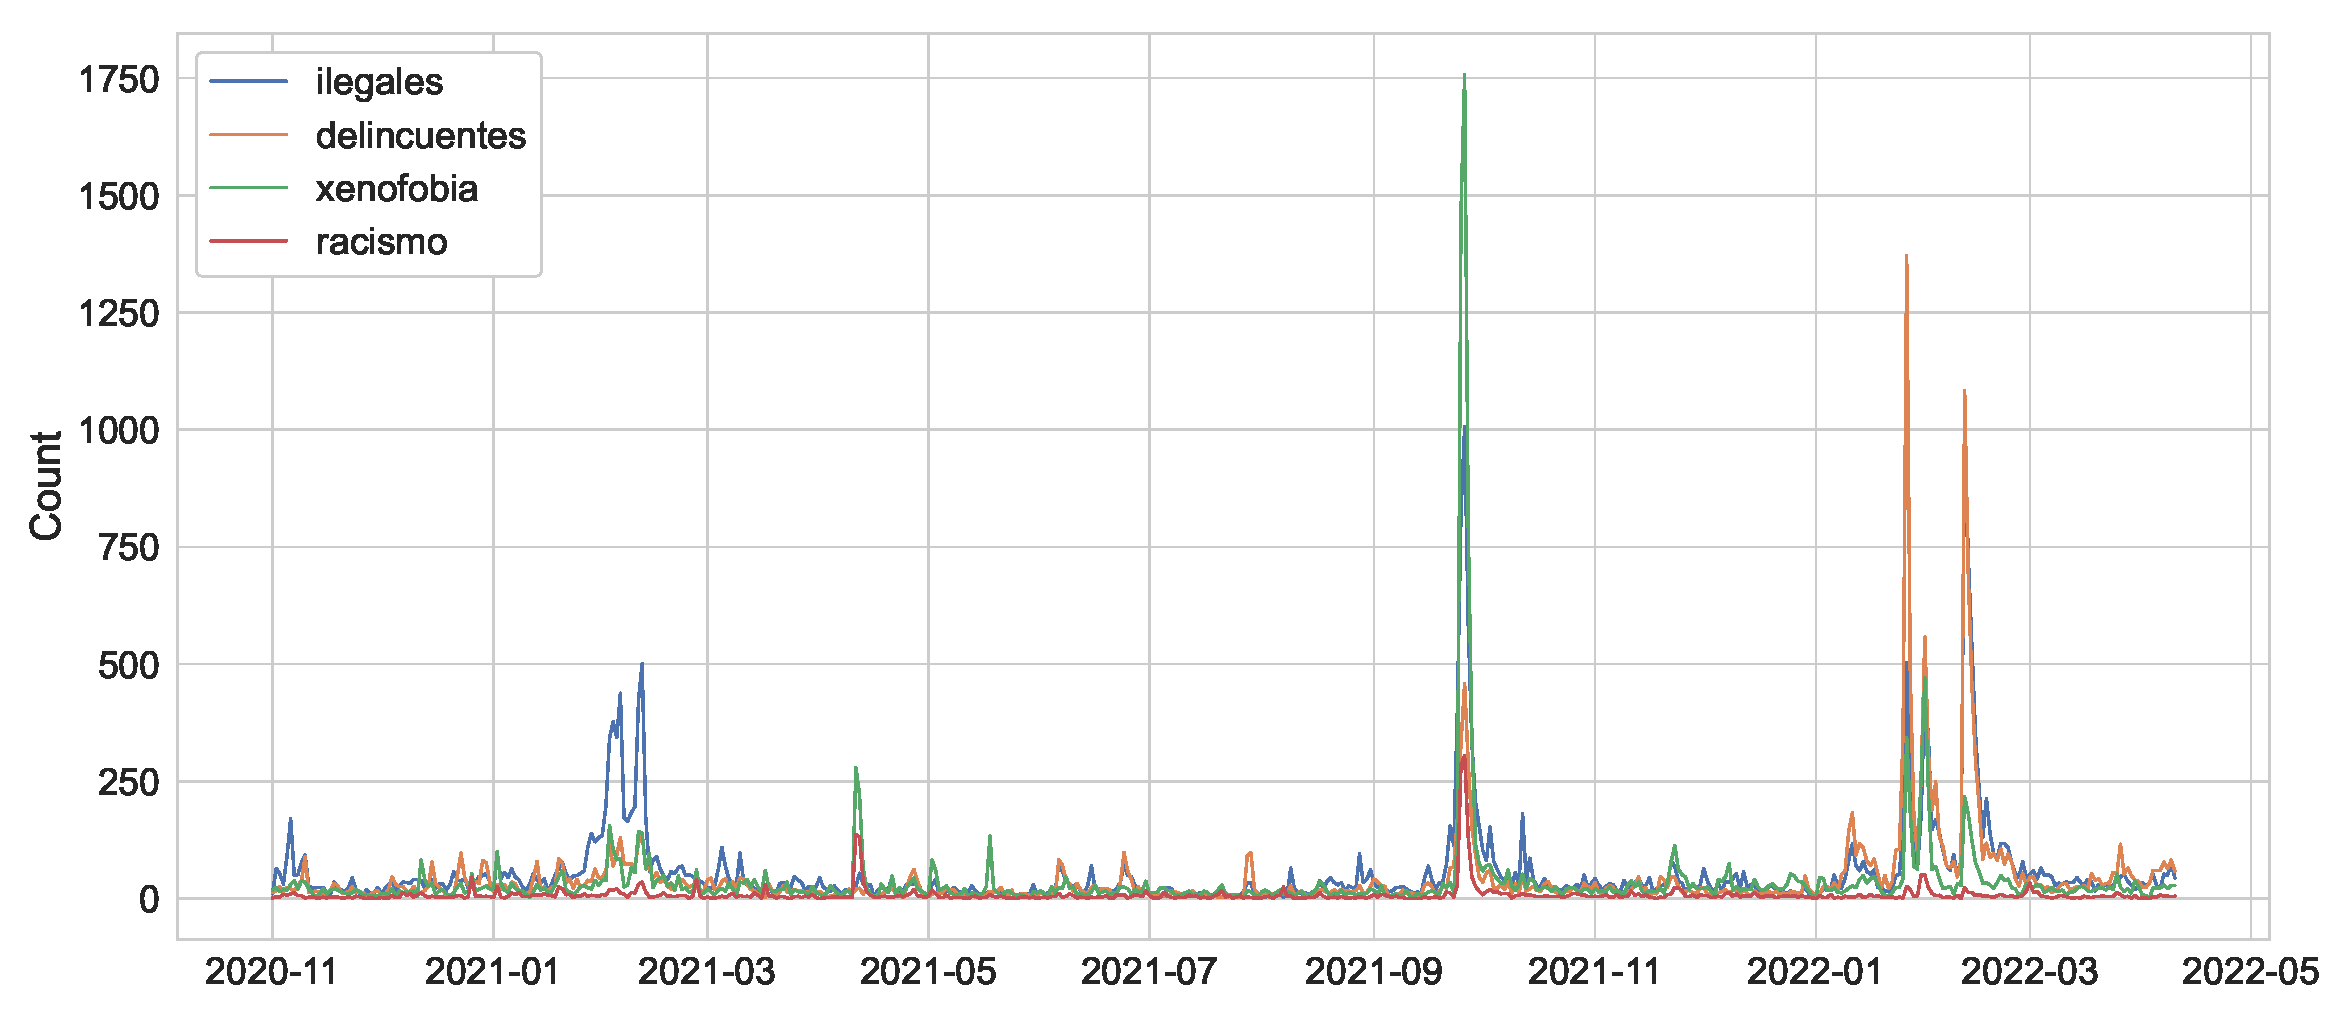
\includegraphics[width=\textwidth]{figs/words_over_time.eps}
             \caption{Usage of Anti-Immigration and Anti-Xenophobia Terms; Total Corpus}
             \label{fig_words_over_time}
             \floatfoot{\it 
                    Notes:  The anti-immigration terms plotted are {\it ‘ilegales’} (Eng: Illegals) and {\it ‘delincuentes’} (Eng: Criminals). The anti-xenophobia terms are {\it ’xenofobia’} (Eng: Xenophobia) and {\it 'racismo'} (Eng: Racism). See Appendix Figure \ref{fig_words_over_time_log} for the same figure in logs. Textual preprocessing steps in outputs include lowercase enforcement and converting Spanish special characters (e.g. á, ñ, etc.) into corresponding non-accentuated ones.
                    \vspace{0.5em} \\
                    Data Source: Retrieved from Twitter API, spanning the time frame Nov 1\textsuperscript{st}, 2020 -- April 11\textsuperscript{th}, 2022. Corpus includes tweets by Twitter users in Chile or Chilean nationals that mainly pertain to immigration. Corpus cleaned by the steps in our methodology as described in Section \ref{sec_meth_gene} and Appendix \ref{app_sec_meth}.}
        \end{figure}
        
        
        